\subsubsection{\newrevision{Mechanical Enclosure and Sensor Pad}}
\label{sec:enclosure_design}
\begingroup\color{green!45!black}
The enclosure design separates the electronics box from a trunk-contact sensor pad. Figures~\ref{fig:enclosure_layout} and~\ref{fig:enclosure_pad} show renders of the proposed geometry. The dimensions below are nominal CAD values.

\begin{table}[htbp]
\centering\small\color{green!45!black}
\caption{\newrevision{Nominal enclosure dimensions.}}
\begin{tabular}{p{0.20\linewidth}p{0.38\linewidth}p{0.32\linewidth}}
\toprule
Part & Dimensions (mm) & Function \\
\midrule
Body & $121\times117\times44.5$; width 165 with flanges & Side-by-side electronics bays \\
Lid & $123\times119\times3$ plate; 14 mm clip arms & Removable snap-fit cover \\
Pad housing & Diameter 56, depth 18; width 88 with ears & Separate 35 mm disc mount \\
\bottomrule
\end{tabular}
\end{table}

The ESP32 and power-assembly bays are on one level, with nominal 1 mm lateral clearance and 7 mm headroom above the assumed 35 mm assemblies. Low ribs locate the boards, and a notch routes the power OUT+ wire towards the ESP32 input. A separate bay protects the sensor module and its prongs; only the disc pad and cable are external. The LoRa bay is a $32\times29$ mm placeholder and must be checked against the actual SX1278 board.

\begin{figure}[htbp]
\centering
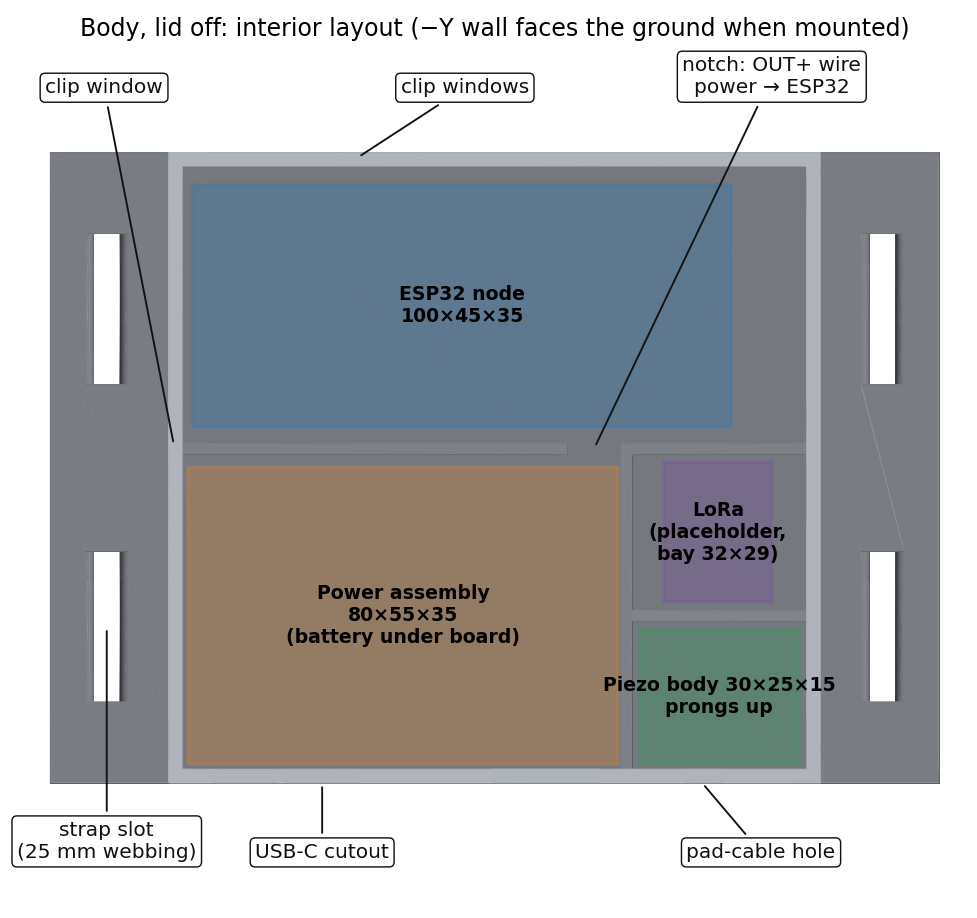
\includegraphics[width=0.49\linewidth]{figures/enclosure/01_interior_layout.png}\hfill
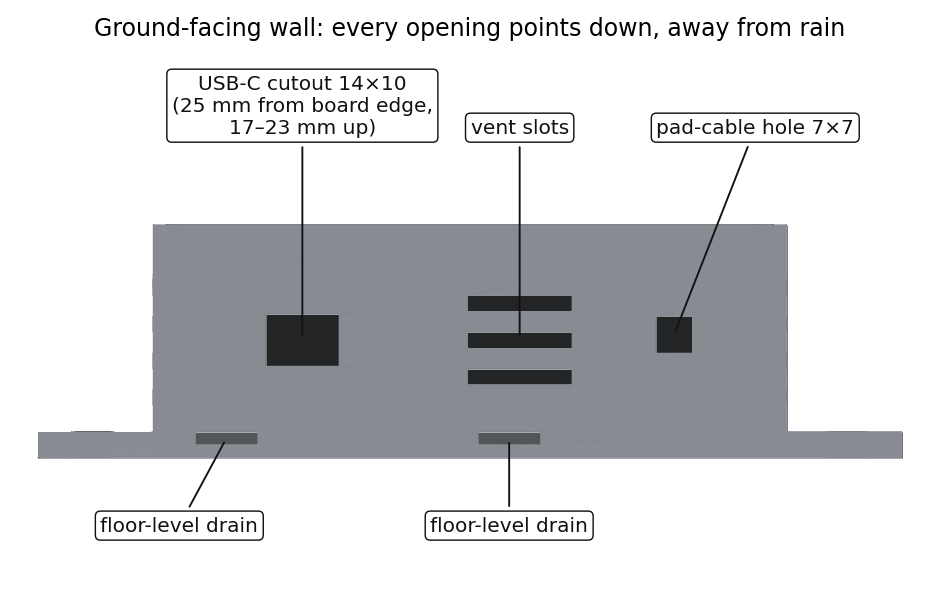
\includegraphics[width=0.49\linewidth]{figures/enclosure/02_ground_wall_openings.png}
\caption{\newrevision{Enclosure CAD renders: component layout (left) and ground-facing USB-C, cable, vent and drain openings (right). Board blocks represent assumed envelopes.}}
\label{fig:enclosure_layout}
\end{figure}
\FloatBarrier

The floor faces the trunk and the lid faces outward for access. Four flange slots accept 25 mm webbing for two retaining straps. The USB-C and sensor-cable openings face downward; side and lower vents provide ventilation, with insect mesh proposed behind them. Two floor-level drains allow water to escape. The lid has four snap arms, a locating lip and a small overhang. This is a ventilated design, not a sealed or IP-rated enclosure; weather resistance, drainage and condensation behaviour require testing.

The pad has its own strap so that the electronics box does not hang from the sensor cable. Its nominal 36 mm pocket accommodates a 35 mm disc on an assumed 8 mm foam backing, leaving the disc about 1.5 mm proud. A foam ring is intended to limit wind exposure while retaining surface contact. The effects of foam, strap pressure and housing mass on sensitivity and background pickup remain experimental questions.

\begin{figure}[htbp]
\centering
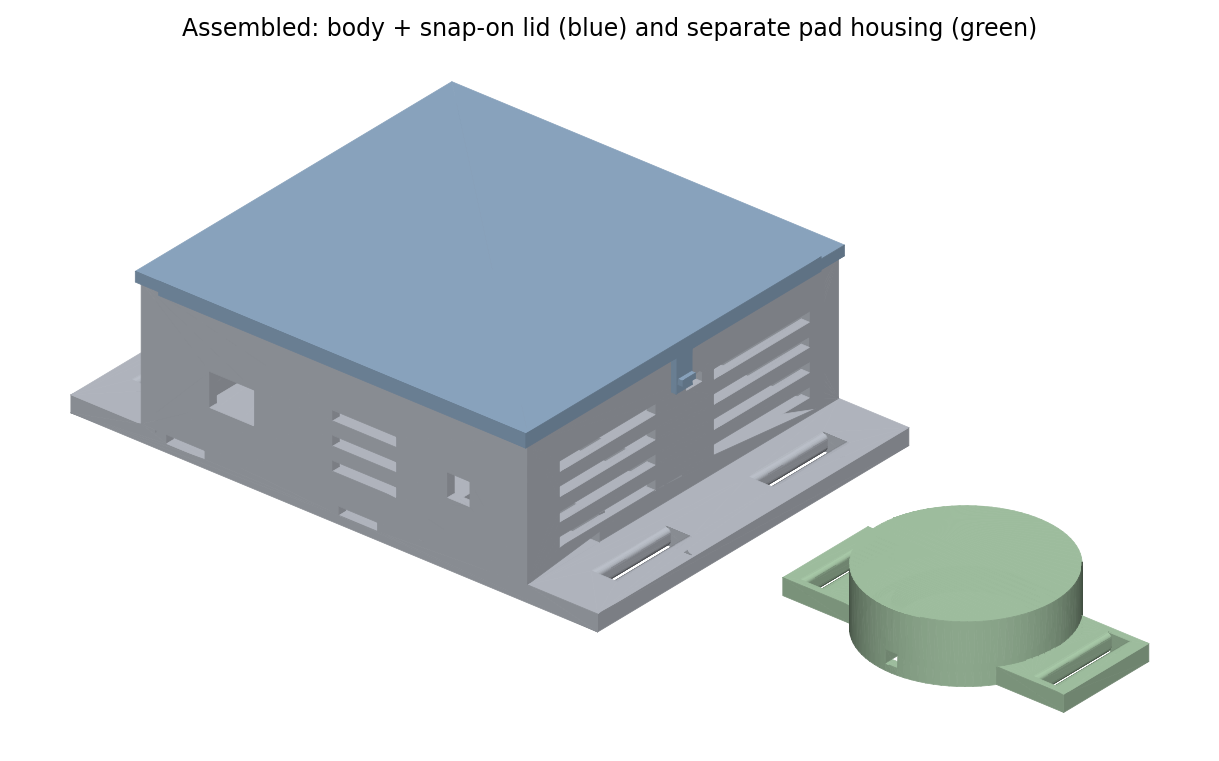
\includegraphics[width=0.49\linewidth]{figures/enclosure/03_assembled_iso.png}\hfill
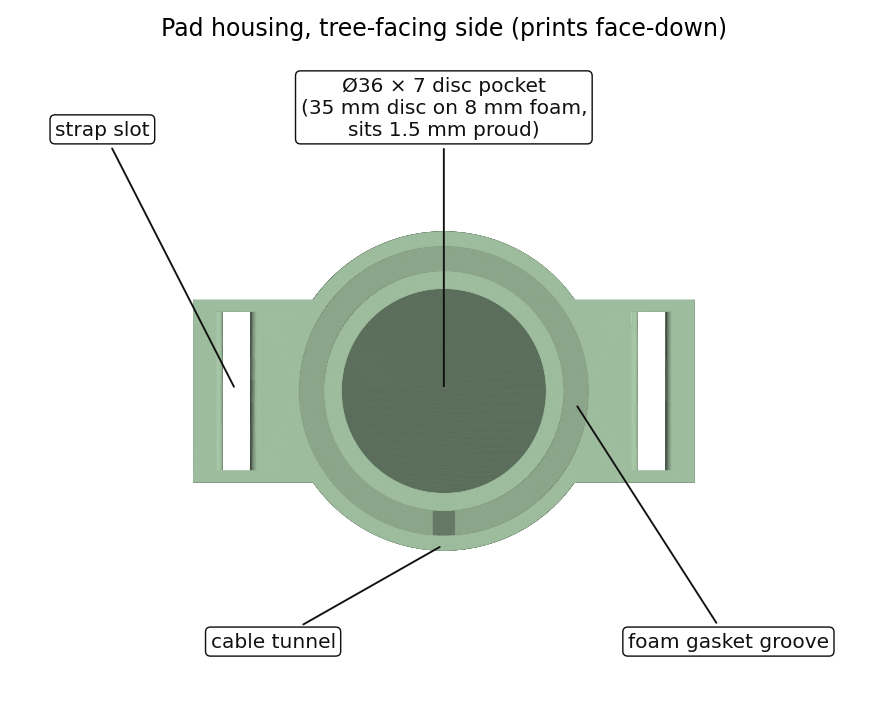
\includegraphics[width=0.49\linewidth]{figures/enclosure/05_pad_housing_face.png}
\caption{\newrevision{CAD renders of the assembled box with separate pad (left) and the pad's disc pocket, foam-ring groove and cable tunnel (right). Acoustic isolation and contact performance have not been measured.}}
\label{fig:enclosure_pad}
\end{figure}
\FloatBarrier
\endgroup
